\documentclass[../main.tex]{subfiles}

\begin{document}

\chapter{June $13^{th} / 2025$}
\label{ch:tufte-design}

\newthought{Multimodal learning of noncoding variant effects using genome sequence and chromatin structure} \cite{10.1093/bioinformatics/btad541}

\hrulefill

$\blacktriangleright$ DL framework to predict the effects of noncoding genetic variants by integrating $1D$ local genome sequence and $3D$ global chromatin structure.
Mathematical architecture overcomes challenges of multimodal data integration (e.g., significance difference in data resolution)

\textbf{\textit{1D Sequence and Epigenetic data}} from DeepSEA (already processed). $5.2 *10^6$ samples where each sample is $1kb$ DNA sequence. Each sequence is labeled with $919$ binary values corresponding to epigenetic effects across $148$ cell lines\\

\textbf{\textit{3D Structure data}} was sourced from Hi-C experiments on the ENCODE portal which provides genome-wide chromatin interaction frequency matrices for cell lines GM12878, IMR90, and K562. Matrices reoersent 3D proximity of different genomic regions (100kb resolution).

\subsection{Mathematical Framework}

\begin{center}
    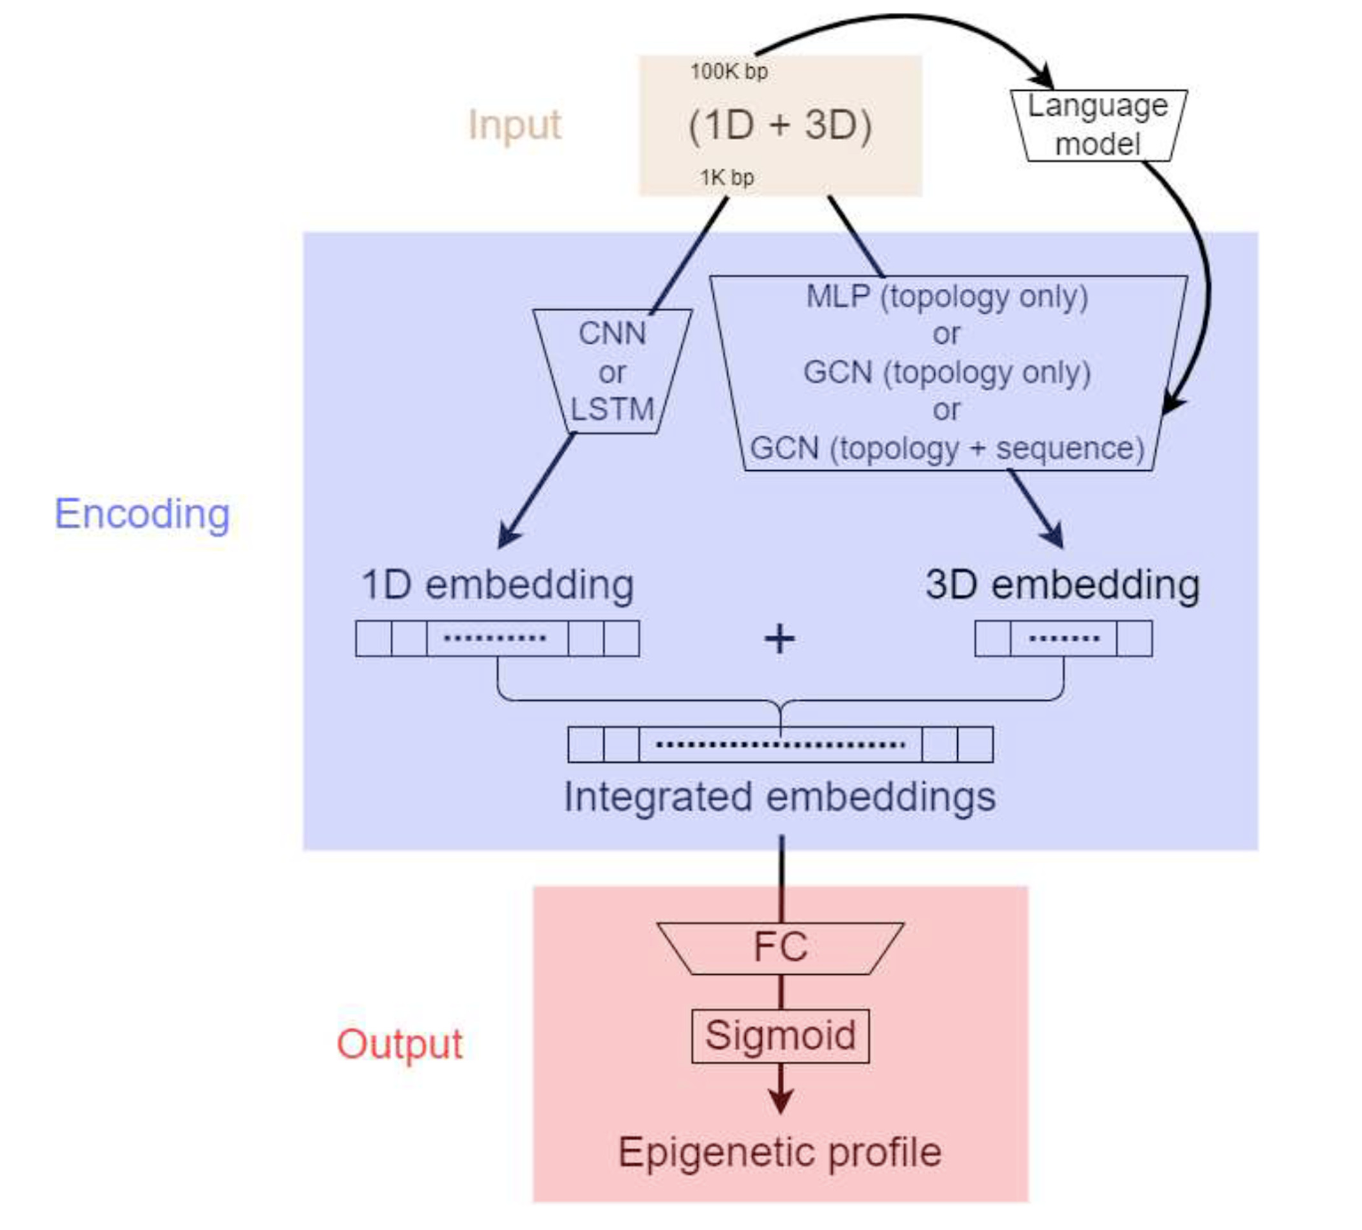
\includegraphics[width=7cm]{files/images/multimodal_nn.png}
\end{center}

\textit{1D Sequence Encoding: CNNs and RNNs ((biLSTM)}

\vspace{0.2cm}

For a $1D$ input sequence $S$ and kernel $K$ of size $k$, the output feature map $C$ at position $i$: 

\[
C_i = f(\sum^k_{j=1} K_j*S_{i+j-1} + b) 
\]
 $f$ is non-linear

and, 
\[
h_{t-1}:h_t=\tanh{(W_{hh}H_{t-1} +W_{xh}x_t+b_h)}
\]

\textit{3D Structure Encoding: GNNs}
\begin{itemize}
    \item GCNs capture complex, non-grid-like topology of chromatin interactions
    \item Feature vector (embedding) $h_i^{l+1}$ for node $i$ at layer $l+1$
\end{itemize}


\[
H^{(l+1)}=\sigma(\Hat{D}^{-\frac{1}{2}}\Hat{A}\Hat{D}^{-\frac{1}{2}}H^{(l)}W^{(l)})
\]

where $H^{(l)}$ is matrix of node features at layer $l$, $\Hat{D}$ is diagonal degree matrix of $\Hat{A}$ and $\Hat{A}=A+I$ (adjacency matrix).

Pre-trained DNA language model used:m \textbf{DNABERT}.

\textit{Training | Prediction}

\vspace{0.3cm}

\textbf{Loss:} Binary cross-entropy. For single data sample:
\[
L = -\sum_{i=1}^{919} \left[ y_i \log(\hat{y}_i) + (1 - y_i) \log(1 - \hat{y}_i) \right]
\]

\textbf{Regularization:} $L1$ and $L2$

\[
\text{L1 penalty: } \lambda_1 \sum |w|
\]
\[
\text{L2 penalty: } \lambda_2 \sum w^2
\]

%%%%%%%%%%%###################
\section{Results}

\textbf{Sequence-only models:} DeepSEA, DanQ, Sei-based model. 

Incorporating $3D$ chromatin structure into model outperforms sequence-only. GCN $+$ DNABERT for structure embedding $\rightarrow$ Improved AUPRC by over $10\%$.

\subsection{Performance Variant Effect Prediction:}
\begin{itemize}
    \item \textbf{eQTL pred.:} Structure-informed models as feature generators yielded better prediction of noncoding variant effects on gene expression vs. sequence-only
    \item \textbf{Pathogenicity pred.:} in \textit{Unsupervised} setting, AUROC $\approx0.75$ and AUPRC $\approx0.15$. In \textit{Supervised} setting (even with $100$ labeled training samples) AUROC $> 0.8$ and AUPRC $>0.25$
\end{itemize}

\subsection{Findings}
\begin{itemize}
    \item $3D$ chromatin structure helps explain disparity between DNA sequence similarity and epigenetic profile similarity. DNA regions far apart in the 1D sequence \textit{but have} similar epigenetic profiles tend to \textit{be closer in 3D space}
    \item Models corrected bias of sequence-only predictors (where sequence similarity was poor indicator of epigenetic similarity)
    \item Using GCNs to embed 3D structure data was \textbf{key strategy}. Chromatin interaction modeled as graphs.
    \item Structure-informed models identified $2$ motifs related to long-range interactions - POU3F1 and TFDP1) which were missed by DanQ BUT at the same time they missed $7$ motifs that DanQ found because they lacked \textbf{long-range interaction patters}
    \item Little to no feature engineering. applicable to multiple types of mutations (insertions, deletions ...) 
    \item DID NOT outperformed CADD in their OWN but when combined
\end{itemize}

$\blacktriangleright$ $7$ motifs missed that were found by sequence-only DanQ likely because motifs lacked long-range interactions that Hi-C data captures. \textit{Using higher-resolution chromatin structure data e.g., from \textbf{Micro-C} experiments, may help.}

\hrulefill

\newthought{Standards and Guidelines for the Interpretation of Sequence
Variants: A Joint Consensus Recommendation of the American
College of Medical Genetics and Genomics and the Association
for Molecular Pathology} \cite{Richards2015}

\hrulefill

$\blacktriangleright$ Framework for standardizing interpretation and classification of genetic variants for Mendelian diseases. 

\textbf{Goal:} To create robust, evidence-based system for consistent variant classification in a clinical context. 

\section{5-Tier Classification System}
\begin{itemize}
    \item \textbf{Pathogenic}
    \item \textbf{Likely Pathogenic}**
    \item \textbf{Uncertain Significance (VUS)}
    \item \textbf{Likely Benign}**
    \item \textbf{Benign}
\end{itemize}

\textbf{**} Represent $> 90\%$ 

\vspace{0.2cm}

\textit{A Variant of Uncertain Significance (VUS) should not be used in clinical decision-making and efforts should be made to resolve its classification}

\section{Evidence Framework} 
For combining different types of evidence to arrive at x classification. Authors chose a rule-based system for combining evidence codes instead of numerical scoring system. Exact numerical relationships cannot be proved yet. Given that the impact of a piece of evidence is often context-dependent they would fail to capture context.

\subsection{Pathogenic Evidence Strengths:}
\begin{itemize}
    \item \textbf{PVS1 (very strong)} Predicted Null variant (e.g., nonsense, frameshift) in a gene where loss of function is a known mechanism of 
    \item \textbf{PS1-PS4 (strong)} Includes evidence like a variant being previously established pathogenic missense variant, confirmed de novo variant in patient with consistent phenotype or variant showing statistically significant increased prevalence in affected individuals vs. controls
    \item \textbf{PM1-PM6 (Moderate)} Includes evidence e.g., being located in a mutational hotspot, being absent from controls in population databases (e.g., ExAC, 1000 Genomes) or being detected \textit{in trans} with another pathogenic variant for a recessive disorder 
    \item \textbf{PP1-PP5 (Supporting)} Evidence like co-segregatuin with disease in a faimily, multiple lines of a computational evidence (tools like SIFT, PolyPhen-2) supporting a damaging effect or a patient's phenotype being highly specific for the gene
\end{itemize}

\subsection{Benign Evidence Strengths}
\begin{itemize}
    \item \textbf{BA1(Stand-Alone)}: Allele frequency is $>5\%$ in a large population database
    \item \textbf{BS1-BS4 (Strong)}: Includes evidence like having an allele frequency greater than expected for x disorder, being observed in a healthy adult for a fully penetrant childhood disease, well established functional studies showing no damaging effect. 
    \item \textbf{Supporting}: Includes evidence like being a missense variant in a gene where only truncating variants are known to cause disease or multiple computational tools suggesting no impact
\end{itemize}

\subsection{Classification Rules | 'Algorithm Classifier'}

\begin{table}[h!]
\centering
\caption{Rules for Combining Criteria to Classify Sequence Variants}
\label{tab:acmg_rules_populated}
\begin{tabular}{p{0.95\textwidth}} % Using a parbox-like column to allow text wrapping and lists
\toprule
\textbf{Pathogenic} \\
\begin{enumerate}[label=\arabic*., wide, labelindent=0pt, topsep=2pt, itemsep=1pt]
    \item 1 Very Strong (PVS1) \textbf{AND} one of the following:
    \begin{enumerate}[label=(\alph*), leftmargin=*, topsep=1pt]
        \item $\ge$1 Strong (PS1--PS4)
        \item $\ge$2 Moderate (PM1--PM6)
        \item 1 Moderate (PM1--PM6) \textbf{AND} 1 Supporting (PP1--PP5)
        \item $\ge$2 Supporting (PP1--PP5)
    \end{enumerate}
    \item $\ge$2 Strong (PS1--PS4)
    \item 1 Strong (PS1--PS4) \textbf{AND} one of the following:
    \begin{enumerate}[label=(\alph*), leftmargin=*, topsep=1pt]
        \item $\ge$3 Moderate (PM1--PM6)
        \item 2 Moderate (PM1--PM6) \textbf{AND} $\ge$2 Supporting (PP1--PP5)
        \item 1 Moderate (PM1--PM6) \textbf{AND} $\ge$4 Supporting (PP1--PP5)
    \end{enumerate}
\end{enumerate}
\vspace{0.5em} \\ 
\midrule

\textbf{Likely Pathogenic} \\
\begin{enumerate}[label=\arabic*., wide, labelindent=0pt, topsep=2pt, itemsep=1pt]
    \item 1 Very Strong (PVS1) \textbf{AND} 1 Moderate (PM1--PM6)
    \item 1 Strong (PS1--PS4) \textbf{AND} 1--2 Moderate (PM1--PM6)
    \item 1 Strong (PS1--PS4) \textbf{AND} $\ge$2 Supporting (PP1--PP5)
    \item $\ge$3 Moderate (PM1--PM6)
    \item 2 Moderate (PM1--PM6) \textbf{AND} $\ge$2 Supporting (PP1--PP5)
    \item 1 Moderate (PM1--PM6) \textbf{AND} $\ge$4 Supporting (PP1--PP5)
\end{enumerate}
\vspace{0.5em} \\
\midrule

\textbf{Benign} \\
\begin{enumerate}[label=\arabic*., wide, labelindent=0pt, topsep=2pt, itemsep=1pt]
    \item 1 Stand-Alone (BA1) \textbf{OR}
    \item $\ge$2 Strong (BS1--BS4)
\end{enumerate}
\vspace{0.5em} \\
\midrule

\textbf{Likely Benign} \\
\begin{enumerate}[label=\arabic*., wide, labelindent=0pt, topsep=2pt, itemsep=1pt]
    \item 1 Strong (BS1--BS4) \textbf{AND} 1 Supporting (BP1--BP7) \textbf{OR}
    \item $\ge$2 Supporting (BP1--BP7)
\end{enumerate}
\vspace{0.5em} \\
\midrule
\multicolumn{1}{p{0.95\textwidth}}{\textit{Variants should be classified as Uncertain Significance if other criteria are unmet or the criteria for benign and pathogenic are contradictory.}} \\
\bottomrule
\end{tabular}
\end{table}


\end{document}